\newcommand{\RN}[1]{%
  \textup{\uppercase\expandafter{\romannumeral#1}}%
}

\Lecture{Jayalal Sarma}{Oct 19, 2020}{17}{Generating Functions(continued)}{Lalithaditya}{$\alpha$}{JS}

\section{Quick Recap of Previous Two Lectures}
 
\begin{itemize}
	\item We represented the sequence of non-negative integers in the form of a formal power series.
	\item Operations on power series corresponding to combinatorial meanings.
	\item We used the concept of Generating Functions for the following examples:
		\begin{enumerate}
			\item Distributing 'n' votes to 'k' candidates such that every candidate gets atleast one vote.
			\item Count the number of non-negative solutions for the equation $a+b+c=n$
			\item Derving the expression for Catalan numbers.
		\end{enumerate}		 
\end{itemize}

\section{Recurrence Relations}

There are three types of recurrence relations,that are being discussed in this lecture. There are Linear Recurrence Relations, Degree Recurrence Relations and Homogenous Recurrence Relations.\\ \ Before getting into examples,lets discuss about these relations.

\begin{itemize}
	\item \textbf{Linear Recurrence Relation:}\\ \\A Linear Recurrence Relation is a equation that defines  $n\textsuperscript{th}$ in a sequence in terms of the $k$ previous terms in the sequence. The recurrence relation is in the form:\\$$a_n = c_1.a_{n-1}~+~c_2.a_{n-2}~+~c_3.a_{n-3}~+~\dots~+~ c_k.a_{n-k}$$ $$ =\sum_{i=1}^{k} c_i*a_{n-i}$$ $where~c_i's~are~constants~independent~of~n$,\\ $c_1,c_2,c_3,\dots,c_k \in \mathbb{R} $ and $c_k \neq 0$.
	
	\item \textbf{Degree Recurrence Relation:}\\ \\A recurrence relation of degree d is said to be Degree Recurrence Relation where $a_n$ depends only on $a_{n-d}$.
	
	\item \textbf{Homogenous Recurrence Relation:}\\ \\ A recurrence relation where each term of the right hand side of the equation has the same degree.
		
	\item \textbf{Some examples on recurrence relations:}
	\begin{enumerate}
		\item $a_n = 5.a_{n-1}~+~a_{n-2}.a_{n-3}$ : This is neither linear nor homogenous.
		\item $a_n = a_{n-1}.a_{n-2}~+~a_{n-3}.a_{n-4}$ : This is not linear but homogenous of degree 4.
		\item $a_n = 5.a_{n-2}~+~10^n$ : This is linear but not homogenous of degree 2.
	\end{enumerate}
\end{itemize}

\section{Using Generating Functions to solve recurrence relations}

In this section, we will look how to solve recurrence relations using generating functions.
\\ \\
\textbf{Example 1:}\\
In the previous lectures,we can calculated the number of binary strings of length n, which have even number of $0$'s. It turned out to be $2^{n-1}$.\\
Similarly, calculate the number of decimal strings of length n, which contain even number of $0$'s.\\ \\
\textbf{Solution:}\\
Let the $a_n$ be the number of decimal strings,which satisfy the given condition.\\
By convention,lets take that when $n=0$, the number of such strings is 1.\\
If $n=1$,then the number of such strings will be 9.\\
$\implies a_0=1$ and $a_1=9$.\\ \\
\textbf{Forming the recurrence relation:}
Let's take a n-length decimal string, and let $d_n$ be the last digit in the string. There are two cases for this type of situation i.e. if $d_n=0$ and $d_n \neq 0$.\\
\underline{\textbf{Case-\RN{1}:}} \\If the last digit is 0, then the remaining string must have odd number of zeroes.Then the number of such strings will be $(10^{n-1} - a_{n-1})$.\\ \\
\underline{\textbf{Case-\RN{2}:}}\\
If the last digit is not zero, then the remaining string must have even number of zeroes,which is equal to number of such strings of length $n-1$ i.e. $a_{n-1}$. The last digit can vary from $1,2,3, \dots,9$. Therefore, the number of such strings will be $(9a_{n-1})$.\\ \\
The resultant recurrence relation for $a_n$ is,\\
$$\implies a_n~=~(10^{n-1}-a_{n-1}+9a_{n-1})$$
$$\implies a_n~=~(10^{n-1}+8a_{n-1})$$
The generating function for this problem will be,
\begin{equation}
G(x) = \sum_{n \geq 0} a_n.x^n
\end{equation}
$$ G(x)~=~a_0~+~\sum_{n \geq 1}a_n.x^n $$
$$ G(x)~=~a_0~+~\sum_{n \geq 1}.(10^{n-1}+8a_{n-1})x^n$$
$$ G(x)~=~1~+~\sum_{n \geq 1} 8.a_{n-1}.x^n~+~\sum_{n \geq 1}10^{n-1}.x^n $$

$$ G(x)~=~1~+~8.x ~\sum_{n \geq 1} a_{n-1}.x^{n-1}~+~x~ \sum_{n \geq 1}10^{n-1}.x^{n-1} $$

Let $n-1~=~h$.Then,

$$ G(x)~=~1~+~8.x ~\sum_{h \geq 0} a_{h}.x^{h}~+~x~ \sum_{h \geq 0}10^{h}.x^{h} $$

After renaming the variable, we have

$$ G(x)~=~1~+~8.x ~\sum_{n \geq 0} a_{n}.x^{n}~+~x~ \sum_{n \geq 0}10^{n}.x^{n} $$

From the equation (17.72), we can see that $G(x) = \sum_{n \geq 0} a_n.x^n$

$$ G(x)~=~1~+~8.x.G(x)~+~x~ \sum_{n \geq 0}10^{n}.x^{n} $$

$$ G(x)~=~1~+~8.x.G(x)~+~x~ \sum_{n \geq 0}{(10.x)}^{n} $$

From the summation of infinte geometric progression, we have

$$\sum_{n \geq 0}{(10.x)}^{n} = \frac{1}{1-10.x}$$

$$ G(x)~=~1~+~8.x.G(x)~+~x.\left(\frac{1}{1-10.x}\right) $$

After rearranging the terms, we finally $G(x)$ as,

$$G(x)~=~\frac{\left(1-9.x\right)}{(1-8.x).(1-10.x)}$$

By using the concept of partial fractions, let's split the above into two fractions,

$$\frac{\left(1-9.x\right)}{(1-8.x).(1-10.x)} ~=~ \frac{A}{(1-8.x)}~+~\frac{B}{(1-10.x)}$$

$$=~\frac{A+B-(10.A.x)-(8.B.x)}{(1-8.x).(1-10.x)}$$

$$\implies A+B=9~and~10.A+8.B=9$$

After solving for A and B, we get $A=\frac{1}{2}$ and $B=\frac{1}{2}$

\begin{equation}
	G(x)~=~\frac{\frac{1}{2}}{(1-8.x)}~+~\frac{\frac{1}{2}}{(1-10.x)}
\end{equation}

Our aim was to find the number $a_n$,which is nothing but the coefficient of $x^n$ in $G(x)$.

$$\implies Coefficient~of~x^n~in~G(x)~=~ \left(\frac{1}{2}.8^n\right) + \left(\frac{1}{2}.10^n\right)$$
$$\hspace{1ex}=~\frac{8^n+10^n}{2}$$

$\therefore$ Number of decimal strings with even number of zeroes is $\left(\frac{8^n+10^n}{2}\right)$.
\\ \\
\textbf{Example 2:}\\
In this example, we are not using any recurrence relations. We are proving combinatorial equations using generating functions.
\\ \\
For $n \geq k$, prove that 
\begin{equation}
	\sum_{m=k}^{k}{m \choose k}~=~{n+1 \choose k+1}
\end{equation}
\textbf{Solution:}\\

For a fixed $k$, lets assume that $$a_n~=~\sum_{m=k}^{n}{m \choose k} $$

The generating function for this problem will be,

\begin{equation}
 S(x)~=~ \sum_{n \geq k}a_n.x^n
\end{equation}

We can observe that in the above summation, n starts from k. It can also start from n = 0, but it is the same, as $k \geq 0$. \\ \\
Lets introduce a new function $\sigma$,

$$ \sigma = \left\{
\begin{array}{ll}
      1 & if~k\leq m\leq n \\
      0 & otherwise \\
\end{array} 
\right. $$

From equation (17.74),

$$ S(x)~=~ \sum_{n \geq k}a_n.x^n$$

$$ S(x)~=~ \sum_{n \geq k}~\sum_{m=k}^{n}{m \choose k}.x^n$$

$$ S(x)~=~ \sum_{n \geq k}\left(~\sum_{m \geq k}{m \choose k}.x^n\left(\sigma \right) \right)$$

After rearranging the summations,

$$ S(x)~=~ \left(~\sum_{m \geq k}\sum_{n \geq k}{m \choose k}.x^n\left(\sigma \right) \right)$$

Since ${k \leq m}$ and ${k \leq n}$ the new function $\sigma$ becomes $1$.\\ \\
Also ${k \leq m}$ and ${k \leq n}$, $\implies m \leq n$.

$$\implies~S(x)~=~ \left(~\sum_{m \geq k}\sum_{n \geq m}{m \choose k}.x^n \right)$$

Since, ${m \choose k}$ is independent of $n$,

$$S(x)~=~ \left(~\sum_{m \geq k}{m \choose k}. \sum_{n \geq m}x^n \right)$$

$$S(x)~=~\sum_{m \geq k}{m \choose k}.\left(x^m \sum_{n \geq m}x^{n-m} \right) $$

We can observe that the second summation is the sum of an infinite geometric progression.

$$S(x)~=~\sum_{m \geq k}{m \choose k}.\left( \frac{x^m}{1-x} \right)$$

\begin{equation}
	S(x)~=~\frac{x^k}{1-x} \left(\sum_{m \geq k} {m \choose k}.x^{m-k} \right)
\end{equation}

We know that,
$$\frac{1}{1-x} = 1+x+x^2+\dots + \dots$$

and also,

$${\left(\frac{1}{1-x}\right)}^{k+1} = {(1+x+x^2+\dots+\dots)^{k+1}} $$

$${(1+x+x^2+\dots+\dots)^{k+1}} = (1+x+x^2+\dots).(1+x+x^2+\dots).\dots $$

Let $d_1,d_2,d_3,\dots,d_{k+1}$ be the degree of each x terms in the product.\\
Our aim is to get the coefficient of $x^{m-k}$ in the above product, this is equivalent to the question \\ \\
\emph{In how many ways can we pick $d_1,d_2,\dots,d_{k+1}$ such that} $$\sum_{i=1}^{k+1}d_i = (m-k)$$\\
This is an example of multichoosing. As discussed in the previous lectures, the number of solutions to this question is $${{k+1+m-k-1} \choose {m-k}} = {m \choose m-k}$$

and also,

$${m \choose m-k} = {m \choose k} $$

From the equation (17.76), we can replace ${m \choose k}.x^{m-k}$ with ${\left(\frac{1}{1-x}\right)}^{k+1}$

$$S(x)~=~\frac{x^k}{1-x}{\left(\frac{1}{1-X} \right)}^{k+1} $$

\begin{equation}
 S(x)~=~\frac{x^k}{{\left(1-x \right)}^{k+2}}
\end{equation}

Our aim is to find the number $a_n$, which is nothing but the coefficient of $x^n$ in the generating function $S(x)$.\\ \\

We can observe that the,

$$Coefficient~of~x^n~in \frac{x^k}{{\left(1-x \right)}^{k+2}}~~=~~Coefficient~of~x^{n-k}~in~{\left(\frac{1}{1-x}\right)}^{k+2}$$

As we proved earlier in this example, that the coefficient of $x^{n-k}$ in the right hand side, is equivalent to the sum of degrees of x terms by expanding $\left(\frac{1}{1-x}\right)$ equal to $(k+2)$.
\\
As proved in earlier lectures, this sum is equal to 

$$a_n = {{k+2+n-k-1} \choose {n-k}}$$

$${{k+2+n-k-1} \choose {n-k}} = {n+1 \choose n-k} $$

$${n+1 \choose n-k} = {n+1 \choose k+1}$$

$$\boxed{\therefore a_n = {n+1 \choose k+1}}$$

\Lecture{Jayalal Sarma}{Oct 20, 2020}{18}{Two Variable Generating Functions}{Lalithaditya and Pragnya}{$\alpha$}{JS}

Till now we had discussed Generating Functions with one variable. In this lecture, we are going to discuss Generating Functions with two variables. Such type of Generating functions are known as \textbf{Bivariate Generating Functions}.\\ \\

The general form of the Bivariate Generating functions is,$$G(x,y) = \sum_{n,k \geq 0} a_{n,k}.x^n.y^k$$

These type of generating functions are useful, when dealing combinatorial problems with two variables.\\
Lets try out some examples, to get an idea on how to use Generating Functions with two variables.

\section{Examples based on Bivariate Generating Functions}
\textbf{Example 1:}\\ Prove the binomial theorem in single variable using the two variable generating functions.\\
Binomial Theorem in single variable:
$${\left(1+x\right)}^{n} = \sum_{k=0}^{n}{n \choose k}.x^k$$
\textbf{Solution:}\\

We know that the number of ways of choosing a k-sized subset from n-sized set is equal to ${n \choose k}$.\\

Let the number be $b_{n,k}$.
\\
When $n=0$ , $b_{0,k}~=~0$ and when $k=0$, $b_{n,0}~=~1$.\\
\\
As discussed in previous lectures, we can choose a k-sized subset from n-1 elements or from n elements.
\\
\textbf{Recurrence relation:}
$$b_{n,k} = b_{n-1,k-1} + b_{n-1,k} $$

The generating function for this problem is,
\begin{equation}
B(x,y) = \sum_{n,k \geq 0}b_{n,k}.\left(x^n.y^k \right)
\end{equation}


$$B(x,y) = \sum_{n \geq 0,k=0}b_{n,0}x^n + \sum_{n=0,k \geq 0}b_{0,k}.y^k + \sum_{n,k \geq 1}b_{n,k}.\left(x^n.y^k \right) $$

We know that $b_{0,k} = 0~and~b_{n,0}=1$.

$$B(x,y) = \sum_{n \geq 0,k=0}1. \left( x^n \right) + \sum_{n=0,k \geq 0}0. \left( y^k \right) + \sum_{n,k \geq 1}b_{n,k}.\left(x^n.y^k \right) $$

$$B(x,y) = \sum_{n \geq 0,k=0} \left( x^n \right) + \sum_{n,k \geq 1}b_{n,k}.\left(x^n.y^k \right)$$

By using the recurrence relation,

$$B(x,y) = \sum_{n \geq 0,k=0} \left( x^n \right) + \sum_{n,k \geq 1}b_{n-1,k-1}.\left(x^n.y^k \right) + \sum_{n,k \geq 1}b_{n-1,k}.\left(x^n.y^k \right)$$

We know that,
$$\sum_{n \geq 0}x^n = \frac{1}{1-x} $$

$$B(x,y) = \frac{1}{1-x} + \sum_{n,k \geq 1}b_{n-1,k-1}.\left(x^n.y^k \right) + \sum_{n,k \geq 1}b_{n-1,k}.\left(x^n.y^k \right)$$

$$B(x,y) = \frac{1}{1-x} + \left(x.y\right)\sum_{n,k \geq 1}b_{n-1,k-1}.\left(x^{n-1}.y^{k-1} \right) + x.\sum_{n,k \geq 1}b_{n-1,k}.\left(x^{n-1}.y^k \right)$$

$$B(x,y) = \frac{1}{1-x} + \left(x.y\right)\sum_{n,k \geq 1}b_{n-1,k-1}.\left(x^{n-1}.y^{k-1} \right) + x.\sum_{n,k \geq 1}b_{n-1,k}.\left(x^{n-1}.y^k \right)$$

Let $(n-1)=h~and~(k-1)=p$

$$B(x,y) = \frac{1}{1-x} + \left(x.y\right)\sum_{h,p \geq 1}b_{h,p}.\left(x^{h}.y^{p} \right) + x.\sum_{n,k \geq 1}b_{n-1,k}.\left(x^{n-1}.y^k \right)$$

After renaming of variables,

$$B(x,y) = \frac{1}{1-x} + \left(x.y\right)\sum_{n,k \geq 1}b_{n,k}.\left(x^{n}.y^{k} \right) + x.\sum_{n,k \geq 1}b_{n-1,k}.\left(x^{n-1}.y^k \right)$$

$$B(x,y) = \frac{1}{1-x} + \left(x.y\right)\sum_{n,k \geq 1}b_{n,k}.\left(x^{n}.y^{k} \right) + x.\left(\sum_{n,k \geq 0}b_{n,k}.\left(x^{n}.y^k \right) - \sum_{n \geq 0,k=0}x^n \right)$$

$$B(x,y) = \frac{1}{1-x} + \left(x.y\right)\sum_{n,k \geq 0}b_{n,k}.\left(x^{n}.y^{k} \right) + x.\left(\sum_{n,k \geq 0}b_{n,k}.\left(x^{n}.y^k \right) - \sum_{n \geq 0,k=0}x^n \right)$$

From the equation (18.78),

$$B(x,y) = \frac{1}{1-x} + \left(x.y\right).B(x,y) + x.\left(B(x,y) - \frac{1}{1-x} \right)$$

After rearranging the terms,

$$B(x,y) = 1+x.\left(y+1\right).B(x,y)$$

$$B(x,y) = \frac{1}{1-x.\left(y+1\right)}$$

$\therefore$ The generating function $B(x,y)$ is,

\begin{equation}
	\boxed{B(x,y) = \frac{1}{1-x.\left(y+1\right)}}
\end{equation}

Coefficient of $x^n$ in the Left hand side of the above equation is equal to the coefficient of $x^n$ in the right hand side of the above equation.

Coefficient of $x^n$ in the left hand side $= \sum_{k \geq 0}b_{n,k}.y^k~(\because From~equation~(18.78))$ 
\\

\textbf{Note:} Coefficient of $x^n$ in $\left(\frac{1}{1-ax}\right)$ is $a^n$.\\

$\implies$ Coefficient of $x^n$ in the right hand side $= {\left(1+y \right)}^{n}$\\

Hence,

$$\sum_{k \geq 0}b_{n,k}.y^k = {\left(1+y \right)}^{n} $$

After renaming of variables,

$${\left(1+x \right)}^{n} = \sum_{k \geq 0}b_{n,k}.x^k $$

At the beginning of the proof, we assumed that $b_{n,k} = {n \choose k}$

\begin{equation}
	\boxed{\therefore {\left(1+x \right)}^{n} = \sum_{k \geq 0}{n \choose k}.x^k}
\end{equation}

which completes our proof.
\\ \\
\textbf{Example 2 (Delannoy Numbers):}\\
Consider a nxn grid. Delannoy number D counts the number of paths from the left-bottom corner (0,0) to any other point on the grid (n,m). \\
The path can be reached by only three paths i.e Upward edges(U), Rightward edges(R) and upward forward diagonals(F). Find the Delannoy Number. \\ \\
\textbf{Solution:}\\
Let $d_{n,m}$ be the number of Delannoy paths from (0,0) to (n,m), by using the above edges only.
\\ \\
For example,When n=3 and m=3, then the number of Delannoy paths is 63.

	\begin{figure}[H]
		\centerline{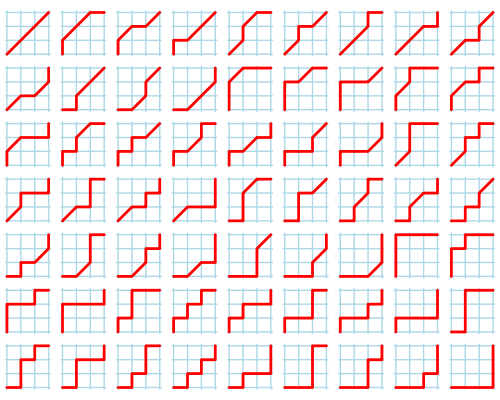
\includegraphics[width=0.5\textwidth,height=0.5\textwidth]{images/DelannoyNumbers.png}}
	\end{figure}
	
\textbf{\underline{Aim}:} To find $d_{n,m}$ \\ 

\textbf{Recurrence Relation:}\\ \\
Lets find a recurrence relation for $d_{n,m}$.
\\ 
A point (n,m) can be reached from three ways i.e. from (n-1,m), from (n-1,m-1) and from (n,m-1).
\\
Hence, the recurrence relation for $d_{n,m}$ will be,
\begin{equation}
\boxed{d_{n,m} = d_{n,m-1} + d_{n-1,m} + d_{n-1,m-1}}
\end{equation}

\textbf{Generating Function:}\\ \\
The generating function for this problem is,
\begin{equation}
\boxed{D(x,y) = \sum_{n,m \geq 0}d_{n,m}.x^n.y^m}
\end{equation}

We can observe that $d_{n,0}=d_{0,m}=1$.

$$D(x,y) = \sum_{n \geq 0,m=0}d_{n,0}.x^n + \sum_{n=0,m \geq 1}d_{0,m}.y^m + \sum_{n \geq 1,m \geq 1}d_{n,m}.x^n.y^m$$

$$D(x,y) = \sum_{n \geq 0,m=0}1.x^n + \sum_{n=0,m \geq 1}1.y^m + \sum_{n \geq 1,m \geq 1}d_{n,m}.x^n.y^m$$

We know that,
$$\sum_{n \geq 0}x^n = \frac{1}{1-x}$$

$$D(x,y) = \frac{1}{1-x} + \sum_{n=0,m \geq 1}y^m + \sum_{n \geq 1,m \geq 1}d_{n,m}.x^n.y^m$$

$$D(x,y) = \frac{1}{1-x} + y.\sum_{n=0,m \geq 1}y^{m-1} + \sum_{n \geq 1,m \geq 1}d_{n,m}.x^n.y^m$$


Let $(m-1)=h$,

$$D(x,y) = \frac{1}{1-x} + y.\sum_{n=0,h=0}y^h + \sum_{n \geq 1,m \geq 1}d_{n,m}.x^n.y^m$$

After renaming the variables,

$$D(x,y) = \frac{1}{1-x} + y.\sum_{n=0,m=0}y^m + \sum_{n \geq 1,m \geq 1}d_{n,m}.x^n.y^m$$

$$D(x,y) = \frac{1}{1-x} + y.\left(\frac{1}{1-y}\right) + \sum_{n \geq 1,m \geq 1}d_{n,m}.x^n.y^m$$

Using the recurrence relation from equation (18.81),

$$D(x,y) = \frac{1}{1-x} + \frac{y}{1-y} + \sum_{n \geq 1,m \geq 1}(d_{n,m-1} + d_{n-1,m} + d_{n-1,m-1}).x^n.y^m$$

$$D(x,y) = \frac{1}{1-x} + \frac{y}{1-y} + \sum_{n \geq 1,m \geq 1}d_{n,m-1} + \sum_{n \geq 1,m \geq 1}d_{n-1,m} + \sum_{n \geq 1,m \geq 1}d_{n-1,m-1}.x^n.y^m$$

$$D(x,y) = \frac{1}{1-x} + \frac{y}{1-y} + x.y.\sum_{n \geq 1,m \geq 1}d_{n-1,m-1}.x^{n-1}.y^{m-1} + \sum_{n \geq 1,m \geq 1}d_{n,m-1} + \sum_{n \geq 1,m \geq 1}d_{n-1,m}$$

Let $(n-1)=h~and~(m-1)=p$,
$$D(x,y) = \frac{1}{1-x} + \frac{y}{1-y} + x.y.\sum_{h \geq 0,p \geq 0}d_{h,p}.x^{h}.y^{p} + \sum_{n \geq 1,m \geq 1}d_{n,m-1} + \sum_{n \geq 1,m \geq 1}d_{n-1,m}$$

After renaming the variables,
$$D(x,y) = \frac{1}{1-x} + \frac{y}{1-y} + x.y.\sum_{n \geq 0,m \geq 0}d_{n,m}.x^{n}.y^{m} + \sum_{n \geq 1,m \geq 1}d_{n,m-1}.x^{n}.y^{m} + \sum_{n \geq 1,m \geq 1}d_{n-1,m}.x^{n}.y^{m}$$

From the equation (18.82),
\begin{equation}
D(x,y) = \frac{1}{1-x} + \frac{y}{1-y} + x.y.D(x,y) + \sum_{n \geq 1,m \geq 1}d_{n-1,m}.x^{n}.y^{m} +\sum_{n \geq 1,m \geq 1}d_{n,m-1}.x^{n}.y^{m}
\end{equation}

Consider the fourth term in the above equation,
$$\sum_{n \geq 1,m \geq 1}d_{n-1,m}.x^{n}.y^{m} = x.\sum_{n \geq 1,m \geq 1}d_{n-1,m}.x^{n-1}.y^{m}$$

Let $(n-1)=h$
$$x.\sum_{n \geq 1,m \geq 1}d_{n-1,m}.x^{n-1}.y^{m} = x.\sum_{h \geq 0,m \geq 1}d_{h,m}.x^h.y^m$$
After renaming the variables,

$$x.\sum_{h \geq 0,m \geq 1}d_{h,m}.x^h.y^m = x.\sum_{n \geq 0,m \geq 1}d_{n,m}.x^n.y^m$$

$$x.\sum_{n \geq 0,m \geq 1}d_{n,m}.x^n.y^m = x.\left(\sum_{n \geq 0,m \geq 0}d_{n,m}.x^{n}.y^{m} - \sum_{n \geq 0,m = 0}d_{n,0}.x^{n} \right)$$

$$x.\left(\sum_{n \geq 0,m \geq 0}d_{n,m}.x^{n}.y^{m} - \sum_{n \geq 0,m = 0}d_{n,0}.x^{n} \right) = x.\left(D(x,y)-\frac{1}{1-x} \right) $$ 
\\ \\
Substituting the above value in the equation (18.83),then

$$D(x,y) = \frac{1}{1-x} + \frac{y}{1-y} + x.y.D(x,y) + x.\left(D(x,y)-\frac{1}{1-x} \right) +\sum_{n \geq 1,m \geq 1}d_{n,m-1}.x^{n}.y^{m}$$

After rearranging the terms,

\begin{equation}
D(x,y) = 1 + \frac{y}{1-y} + x.y.D(x,y) + x.D(x,y) + \sum_{n \geq 1,m \geq 1}d_{n,m-1}.x^{n}.y^{m}
\end{equation}

Consider the last term of the above equation,

$$\sum_{n \geq 1,m \geq 1}d_{n,m-1}.x^{n}.y^{m} = y.\sum_{n \geq 1,m \geq 1}d_{n,m-1}.x^{n}.y^{m-1} $$

Let $p=(m-1)$,then 

$$y.\sum_{n \geq 1,m \geq 1}d_{n,m-1}.x^{n}.y^{m-1} = y.\sum_{n \geq 1,p \geq 0}d_{n,p}.x^{n}.y^{p}$$

After renaming the variables,

$$y.\sum_{n \geq 1,m \geq 0}d_{n,m}.x^{n}.y^{m} = y.\left(\sum_{n \geq 0,m \geq 0}d_{n,m}.x^n.y^m - \sum_{n=0,m \geq 0}d_{0,m}.y^{m} \right) $$

$$y.\left(\sum_{n \geq 0,m \geq 0}d_{n,m}.x^n.y^m - \sum_{n=0,m \geq 0}d_{0,m}.y^{m} \right) = y.\left(D(x,y) - \frac{1}{1-y} \right) $$

Substitute the above value in the equation (18.84),

$$D(x,y) = 1 + \frac{y}{1-y} + x.y.D(x,y) + x.D(x,y) + y.\left(D(x,y) - \frac{1}{1-y} \right)$$

$$D(x,y) = 1 + x.y.D(x,y) + x.D(x,y) + y.D(x,y) $$

After rearranging the terms,

$$D(x,y) = \frac{1}{1-x-y-xy} $$

$$D(x,y) = \left(\frac{1}{1-y}\right).\left(\frac{1}{1-\left(\frac{1+y}{1-y}\right).x}\right) $$

We know that,
$$\frac{1}{1-a.x} = \sum_{n \geq 0}a^n.x^n $$

$$D(x,y) = \left(\frac{1}{1-y}\right).\left(\sum_{n \geq 0}{\left(\frac{1+y}{1-y} \right)}^n.x^n \right) $$

The generating function is,
\begin{equation}
\boxed{D(x,y) = \left(\sum_{n \geq 0}{\frac{{(1+y)}^n}{{(1-y)}^{n+1}}}.x^n \right)}
\end{equation}

The required number $d_{n,m}$ is,\\

$$d_{n,m}~=~Coefficient~of~x^n.y^m~in~D(x,y)$$

$$d_{n,m}~=~Coefficient~of~y^m~in~{\frac{{(1+y)}^n}{{(1-y)}^{n+1}}}$$

$$d_{n,m}~=~Coefficient~of~y^m~in~ {(1+y)}^n.\left(\frac{1}{1-y}.\frac{1}{1-y}. \dots (n+1) times\right)$$

We know that,

$$\frac{1}{1-y} = 1+y+y^2+ \dots$$

$$d_{n,m}~=~Coefficient~of~y^m~in~{(1+y)}^n.\left((1+y+y^2+\dots).(1+y+y^2+\dots). \dots (n+1) times\right)$$

Let's say that a number $k \geq 0$ is taken, such that the term along with its coefficient $y^k$ comes from ${(1+y)^n}$ and the remaining term along with its coefficient $y^{m-k}$ comes from the (n+1) term product.\\

The coefficient of $y^k$ in ${(1+y)^n}$ is ${n \choose k}$.\\

Let $c_1,c_2,\dots,c_{n+1}$ be the degrees of x from the (n+1)-term product.\\

Finding out the coefficient of $y^{m-k}$ from the (n+1) term product is equivalent to count the number of ways of picking $c_i$'s such that $c_1+c_2+\dots+c_{n+1}=m-k$\\

The number of such pickings = ${{n+1+m-k-1} \choose {m-k}}$ = ${n+m-k} \choose {m-k}$ = ${n+m-k} \choose {n}$.\\

Therefore, the required number $d_{n,m}$ is,

$$d_{n,m} = \sum_{k \geq 0}{n \choose k}.{{n+m-k} \choose n}$$

Hence,
\begin{equation}
\boxed{Delannoy~Number~(D) = \sum_{k \geq 0}{n \choose k}.{{n+m-k} \choose n}}
\end{equation}























 

